% Figure: how a vision-language model is wired. (a) image -> vision encoder -> patch vectors -> connector -> visual tokens placed before the text prompt of a decoder-only LM, which generates the answer. (b) two places the LM can read the image: prefix in the sequence vs inserted cross-attention layers. (c) two training stages: which parts are frozen and which are trained.
% Design width ~168mm.
\documentclass[border=0pt]{standalone}
\usepackage{amsmath,amssymb}
% Shared visual language for the figures of the book.
% Every figure in this directory loads this file so the chapter reads as one system.
% NOTE: no blank lines are allowed inside \tikzset{...} (a blank line emits \par
% and breaks key scanning).
\NeedsTeXFormat{LaTeX2e}
\ProvidesPackage{figstyle}[2026/10/21 Figure style for Free Energy to LLMs]

\RequirePackage{tikz}
\usetikzlibrary{arrows.meta,positioning,calc,fit,shapes.geometric,shapes.misc,%
  backgrounds,matrix,decorations.pathreplacing,decorations.markings,patterns.meta}

% ---------------------------------------------------------------- palette
% Same values as book/preamble/style.tex, prefixed with F.
\definecolor{FNavy}{HTML}{14324A}
\definecolor{FTeal}{HTML}{0E7490}
\definecolor{FSky}{HTML}{E7F5F8}
\definecolor{FOrange}{HTML}{D97706}
\definecolor{FAmber}{HTML}{FFF3D6}
\definecolor{FInk}{HTML}{1F2937}
\definecolor{FSlate}{HTML}{64748B}
\definecolor{FMist}{HTML}{F5F7FA}
\definecolor{FRose}{HTML}{9F1239}
\definecolor{FRoseMist}{HTML}{FFF1F2}

% ---------------------------------------------------------------- semantics
% Teal   = probability / model / data object
% Orange = training objective, cost, or the quantity moved through the system
% Navy   = neutral structure
% Slate  = secondary label or metadata
% Rose   = failure mode, hazard, masked-out region
\tikzset{
  % Lay figures out in millimetres.  A figure designed 168mm wide is included at
  % \textwidth, so its fonts appear at exactly the size written here.
  every picture/.style={x=1mm,y=1mm,font=\small,line cap=round,line join=round},
  % ---- block styles
  nbase/.style={draw,rounded corners=1.2pt,align=center,inner sep=2.4pt,%
    minimum height=7mm,text=FInk},
  nteal/.style={nbase,draw=FTeal,fill=FSky},
  norange/.style={nbase,draw=FOrange,fill=FAmber},
  nnavy/.style={nbase,draw=FNavy,fill=white},
  nsoft/.style={nbase,draw=FSlate!55,fill=FMist},
  nrose/.style={nbase,draw=FRose,fill=FRoseMist},
  ghost/.style={draw=none,fill=none,align=center,inner sep=1pt},
  plain/.style={draw=none,fill=none,align=center,inner sep=0pt},
  % ---- arrows
  ar/.style={-{Latex[length=1.7mm,width=1.35mm]},draw=FSlate,line width=0.75pt},
  ard/.style={ar,dashed},
  arteal/.style={ar,draw=FTeal},
  arorange/.style={ar,draw=FOrange},
  arrose/.style={ar,draw=FRose},
  thickar/.style={ar,line width=1.2pt},
  % ---- text roles
  ftitle/.style={font=\large\bfseries,text=FNavy,align=center},
  ptitle/.style={font=\small\bfseries,text=FNavy,align=center},
  ptitleo/.style={font=\small\bfseries,text=FOrange,align=center},
  lbl/.style={font=\scriptsize,text=FSlate,align=center,inner sep=1pt},
  lblt/.style={lbl,text=FTeal},
  lblo/.style={lbl,text=FOrange},
  lbln/.style={lbl,text=FNavy},
  lblr/.style={lbl,text=FRose},
  sub/.style={font=\scriptsize,text=FSlate!90,align=center,inner sep=1pt},
  monob/.style={font=\ttfamily\scriptsize,text=FInk,inner sep=1pt},
  mathb/.style={font=\small,text=FInk,inner sep=1pt},
  eqn/.style={font=\scriptsize,inner sep=1.5pt,text=FInk},
  % ---- decorations
  brace/.style={decorate,decoration={brace,amplitude=2.4pt},draw=FSlate,%
    line width=0.6pt},
  bracet/.style={brace,draw=FTeal},
  braceo/.style={brace,draw=FOrange},
  axis/.style={draw=FSlate!55,line width=0.6pt},
  guide/.style={draw=FSlate!45,line width=0.5pt,dashed},
  halolabel/.style={font=\scriptsize,text=FInk,fill=white,fill opacity=0.85,%
    text opacity=1,inner sep=1.4pt,align=center},
}

% Figure title above the drawing, anchored at the figure's top-left.
\newcommand{\figtitle}[2][0]{%
  \node[ftitle,anchor=north west,outer sep=0pt] at (#1,0) {#2};}

% Rounded panel behind a subgroup of nodes.
\newcommand{\figpanel}[3][]{%
  \node[draw=FSlate!35,fill=#3,rounded corners=2pt,inner sep=2.6mm,#1] {#2};}

\endinput

\begin{document}
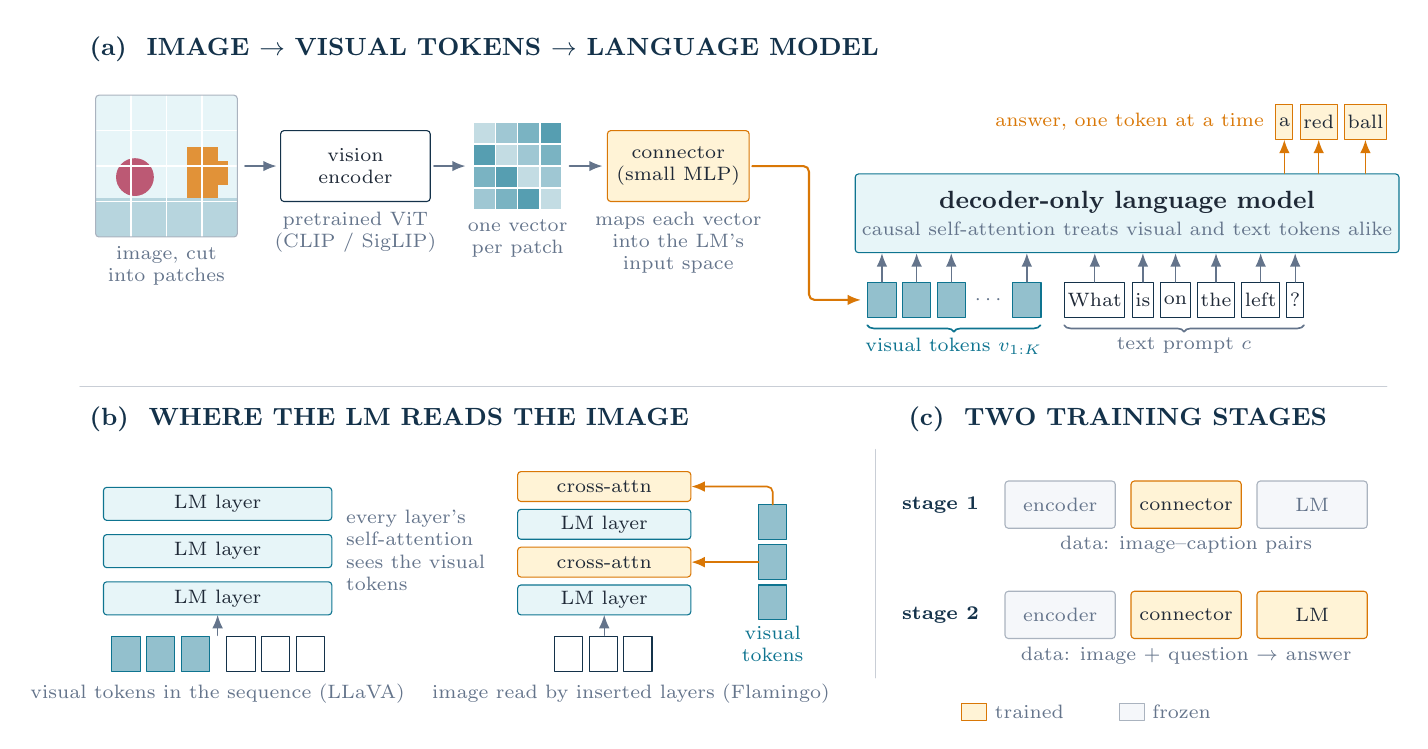
\begin{tikzpicture}[
  vtok/.style={draw=FTeal,fill=FTeal!45,minimum width=3.6mm,minimum height=4.4mm,inner sep=0pt},
  ttok/.style={draw=FNavy,fill=white,minimum height=4.4mm,inner sep=1.1pt,font=\scriptsize,text=FInk},
  atok/.style={draw=FOrange,fill=FAmber,minimum height=4.4mm,inner sep=1.1pt,font=\scriptsize,text=FInk},
  frozen/.style={nsoft,minimum width=14mm,minimum height=6mm,font=\scriptsize,text=FSlate},
  trained/.style={norange,minimum width=14mm,minimum height=6mm,font=\scriptsize},
]
% ======================================================= (a) architecture
\node[ptitle,anchor=south west] at (0,79) {(a)\ \ IMAGE $\to$ VISUAL TOKENS $\to$ LANGUAGE MODEL};
% image with patch grid
\begin{scope}
  \clip[rounded corners=1.2pt] (2,58) rectangle (20,76);
  \fill[FSky] (2,58) rectangle (20,76);
  \fill[FTeal!30] (2,58) rectangle (20,63);
  \fill[FRose!70] (7,65.6) circle (2.4);
  \fill[FOrange!80] (13.6,63) rectangle (17.6,69.4);
  \fill[FOrange!80] (17.6,64.6) rectangle (18.8,67.6);
  \foreach \g in {6.5,11,15.5}{%
    \draw[white,line width=0.6pt] (\g,58)--(\g,76);%
  }
  \foreach \g in {62.5,67,71.5}{%
    \draw[white,line width=0.6pt] (2,\g)--(20,\g);%
  }
\end{scope}
\draw[FSlate!55,rounded corners=1.2pt] (2,58) rectangle (20,76);
\node[lbl,anchor=north] at (11,57.2) {image, cut\\into patches};
\draw[ar] (21,67)--(25,67);
\node[nnavy,minimum width=19mm,minimum height=9mm,font=\scriptsize] at (35,67) {vision\\encoder};
\node[lbl,anchor=north] at (35,61.6) {pretrained ViT\\(CLIP / SigLIP)};
\draw[ar] (45,67)--(49,67);
% patch vectors, one per patch, same layout
\foreach \i in {0,...,3}{%
  \foreach \j in {0,...,3}{%
    \pgfmathsetmacro{\shade}{int(25+15*mod(\i*3+\j*5,4))}%
    \fill[FTeal!\shade] ({50+2.8*\j},{72.6-2.8*(\i+1)}) rectangle ++(2.8,2.8);%
  }%
}
\foreach \g in {0,...,4}{%
  \draw[white,line width=0.6pt] ({50+2.8*\g},61.4)--({50+2.8*\g},72.6);%
  \draw[white,line width=0.6pt] (50,{61.4+2.8*\g})--(61.2,{61.4+2.8*\g});%
}
\node[lbl,anchor=north] at (55.6,60.6) {one vector\\per patch};
\draw[ar] (62.2,67)--(66.4,67);
\node[norange,minimum width=18mm,minimum height=9mm,font=\scriptsize] at (76,67) {connector\\(small MLP)};
\node[lbl,anchor=north] at (76,61.6) {maps each vector\\into the LM's\\input space};
\draw[arorange,rounded corners=2pt] (85.4,67)--(92.6,67)--(92.6,50)--(99.2,50);
% input sequence of the language model
\foreach \x/\n in {100/v1,104.4/v2,108.8/v3,118.4/vK}{%
  \node[vtok,anchor=west] (\n) at (\x,50) {};%
}
\node[lbl] at (115.6,50) {$\cdots$};
\node[ttok,anchor=west] (t1) at (125,50) {What};
\node[ttok,right=0.8mm of t1] (t2) {is};
\node[ttok,right=0.8mm of t2] (t3) {on};
\node[ttok,right=0.8mm of t3] (t4) {the};
\node[ttok,right=0.8mm of t4] (t5) {left};
\node[ttok,right=0.8mm of t5] (t6) {?};
\draw[bracet] (122,46.8)--(100,46.8);
\node[lblt,anchor=north] at (111,45.6) {visual tokens $v_{1:K}$};
\draw[brace] (t6.south east|-0,46.8)--(125,46.8);
\node[lbl,anchor=north] at ($(125,45.6)!0.5!(t6.south east|-0,45.6)$) {text prompt $c$};
% language model
\node[nteal,minimum width=66mm,minimum height=10mm,align=center] (lm) at (133,61)
  {\textbf{decoder-only language model}\\[-0.4mm]{\scriptsize\color{FSlate}causal self-attention treats visual and text tokens alike}};
\foreach \n in {v1,v2,v3,vK,t1,t2,t3,t4,t5,t6}{%
  \draw[ar,line width=0.5pt] (\n.north)--(\n.north|-lm.south);%
}
% generated answer
\node[atok,anchor=east] (a3) at (166,72.6) {ball};
\node[atok,left=0.8mm of a3] (a2) {red};
\node[atok,left=0.8mm of a2] (a1) {a};
\node[lblo,anchor=east] at ($(a1.west)+(-1,0)$) {answer, one token at a time};
\foreach \n in {a1,a2,a3}{%
  \draw[arorange,line width=0.5pt] (\n.south|-lm.north)--(\n.south);%
}
% ======================================================= (b) where the LM reads
\draw[FSlate!35] (0,39)--(166,39);
\node[ptitle,anchor=south west] at (0,32) {(b)\ \ WHERE THE LM READS THE IMAGE};
% b1: prefix
\foreach \x in {4,8.4,12.8}{\node[vtok,anchor=west] at (\x,5) {};}
\foreach \x in {18.6,23,27.4}{\node[ttok,anchor=west,minimum width=3.6mm,inner sep=0pt] at (\x,5) {};}
\foreach \y in {10,16,22}{%
  \node[nteal,minimum width=29mm,minimum height=4.2mm,font=\scriptsize,inner sep=0pt] at (17.5,\y+2.1) {LM layer};%
}
\draw[ar,line width=0.5pt] (17.5,7.4)--(17.5,10);
\node[lbl,anchor=west,align=left] at (33.4,18.2) {every layer's\\self-attention\\sees the visual\\tokens};
\node[lbl,anchor=north] at (17.5,1.6) {visual tokens in the sequence (LLaVA)};
% b2: cross-attention
\foreach \x in {60.2,64.6,69}{\node[ttok,anchor=west,minimum width=3.6mm,inner sep=0pt] at (\x,5) {};}
\node[nteal,minimum width=22mm,minimum height=3.8mm,font=\scriptsize,inner sep=0pt] at (66.6,11.9) {LM layer};
\node[norange,minimum width=22mm,minimum height=3.8mm,font=\scriptsize,inner sep=0pt] (x1) at (66.6,16.7) {cross-attn};
\node[nteal,minimum width=22mm,minimum height=3.8mm,font=\scriptsize,inner sep=0pt] at (66.6,21.5) {LM layer};
\node[norange,minimum width=22mm,minimum height=3.8mm,font=\scriptsize,inner sep=0pt] (x2) at (66.6,26.3) {cross-attn};
\draw[ar,line width=0.5pt] (66.6,7.4)--(66.6,10);
\foreach \y in {11.6,16.7,21.8}{\node[vtok] at (88,\y) {};}
\node[lblt,anchor=north] at (88,9) {visual\\tokens};
\draw[arorange,line width=0.6pt] (86.2,16.7)--(x1.east);
\draw[arorange,line width=0.6pt,rounded corners=2pt] (88,24)--(88,26.3)--(x2.east);
\node[lbl,anchor=north] at (70,1.6) {image read by inserted layers (Flamingo)};
% ======================================================= (c) training stages
\node[ptitle,anchor=south west] at (104,32) {(c)\ \ TWO TRAINING STAGES};
\draw[FSlate!35] (101,2)--(101,31);
\node[lbln,anchor=west,font=\scriptsize\bfseries] at (104,24) {stage 1};
\node[frozen] at (124.5,24) {encoder};
\node[trained] at (140.5,24) {connector};
\node[frozen] at (156.5,24) {LM};
\node[lbl,anchor=north] at (140.5,20.4) {data: image--caption pairs};
\node[lbln,anchor=west,font=\scriptsize\bfseries] at (104,10) {stage 2};
\node[frozen] at (124.5,10) {encoder};
\node[trained] at (140.5,10) {connector};
\node[trained] at (156.5,10) {LM};
\node[lbl,anchor=north] at (140.5,6.4) {data: image + question $\to$ answer};
\fill[FAmber,draw=FOrange] (112,-3.4) rectangle ++(3.2,2.2);
\node[lbl,anchor=west] at (115.8,-2.3) {trained};
\fill[FMist,draw=FSlate!55] (132,-3.4) rectangle ++(3.2,2.2);
\node[lbl,anchor=west] at (135.8,-2.3) {frozen};
\end{tikzpicture}
\end{document}
